%!TEX encoding = UTF-8 Unicode 
%!TEX TS-program = pdflatex

\documentclass[a4paper,12pt,english]{article} 
\usepackage[utf8]{inputenc}
\usepackage{babel}
\usepackage[utf8]{inputenc} 
\usepackage[T1]{fontenc}
\usepackage{indentfirst}
\usepackage{hyperref}
\usepackage{upquote}

\usepackage{pdflscape}
\usepackage{graphicx} 

\graphicspath{{./images/}}


\pagestyle{plain} 
\author{AM27}
\title{Communication protocol}
\date{Software Engineering Project \\
	Academic Year 2019/2020
}


\begin{document}	
	\maketitle
	\newpage
	\tableofcontents
	\newpage
	
	\section{Introduction}
	
	This document specifies the standardized communication protocol used in the group's Santorini project. The protocol is based on the JSON format to allow different applications to read and interpret the various messages and commands. Every message after the connection follows the format:
	\begin{verbatim}
	{ 
	    "type": "TYPE", 
	    "message": "{ 
	        ...
	    }" 
	}
	\end{verbatim}
	Where the type identifies the following message, which needs to be deserialized. The second serialization's details to comply with the JSON format (In particular the escaping of \texttt{"} characters) have been omitted to favour readability.
	
	Once the server accepts a client an heartbeat message system is established (using the type \texttt{PING}), to assure that every party is still active.
	
	\begin{figure}[t]
		\centering	
		{\includegraphics[scale=0.3,keepaspectratio]
			{init.eps}}
		\caption{Example of connection and initialization}
		\label{1hot} 
	\end{figure}
	
	\section{Connection}
	The client connection phase is executed after a client inserts an IP address and port, so the server can be reached. After the ping message the server communicates whether there is a game waiting; consequently the client sends a registration message of type (A) or (B).
	
	%image
	\subsection{serverState}
	Message type: Server $\rightarrow$ Client	
	\begin{verbatim}
	{
	    "type": "SERVERSTATE",
	    "message": "{
	        "open": true,
	        "active": false
	    }"
	}
	\end{verbatim}
	The message contains two boolean values, specifying if the client has been accepted (\texttt{open}) and if there is a match already waiting for players (\texttt{active}).
	
	\subsection{register (A)}
	Message type: Client $\rightarrow$ Server
	\begin{verbatim}
	{
	    "type": "REGISTER",
	    "message": "{
	        "nickname": "PLAYER",
	        "nPlayers": 2,
	        "gods": true
	    }"
	}
	\end{verbatim}
	This message is sent if there is no active game waiting on the server; contains the configuration for the game.
	
	\subsection{register (B)}
	Message type: Client $\rightarrow$ Server
	\begin{verbatim}
	{
	    "type": "REGISTER",
	    "message": "{
	        "nickname": "PLAYER"
	    }"
	}
	\end{verbatim}
	This message is sent if there is already an active game waiting on the server.
	
	\section{Game initialization}
	As per the game's rules, in order to start the game the players must choose a god, then the starter; these operations are done through the following messages.
	%image
	
	\subsection{Choosing a god}
	
	\subsubsection{godList}
	Message type: Server $\rightarrow$ Client	
	\begin{verbatim}
	{
	    "type": "GODLISTMESSAGE",
	    "message": "{
	         "player": "PLAYER",
	         "godList": [
	            {
	                "name": "GOD", 
	                "description": "This god..."
	            },
	            {...}
	        ]
	   }"
	}
	\end{verbatim}
	The message contains the name of the active player and the list of gods that can still be chosen.
	
	\subsubsection{chooseGod}
	Message type: Client $\rightarrow$ Server	
	\begin{verbatim}
	{
	    "type": "GODINIT",
	    "message": "{
	        "player": "PLAYER",
	        "godName": "GOD"   
	    }"
	}
	\end{verbatim}
	This message contains the god chosen by a player.
	
	\subsection{Choosing the starting player}
	
	\subsubsection{players}
	Message type: Server $\rightarrow$ Client	
	\begin{verbatim}
	{
	    "type": "PLAYERSMESSAGE",
	    "message": "{
	        "player": "PLAYER",
	        "players": {
	            ["P1", "GOD1"],
	            ["P2", "GOD2"],
	            ["P3", "GOD3"],
	        }
	    }"
	}
	\end{verbatim}
	This message is sent to everyone to let them know the opponents and their respective gods; the challenger has to choose the starter player from the list.
	
	\subsubsection{chooseStarter}
	Message type: Client $\rightarrow$ Server
	\begin{verbatim}
	{
	    "type": "STARTER",
	    "message": "{
	        "player": "P1",
	        "starter": "P2"
	    }"
	}
	\end{verbatim}
	This is the message sent by the challenger after choosing the starting player.
	\newpage
	\begin{figure}[t]
		\centering	
		{\includegraphics[scale=0.3,keepaspectratio]
			{game.eps}}
		\caption{Example of a normal interaction during a turn}
		\label{1hot} 
	\end{figure}
	
	\section{Game}
	The following sections illustrate the messages exchanged during a game.
	
	\subsection{Server updates}
	The updates sent by the server regulate entirely the clients' behaviour.
	
	\subsubsection{update}
	\begin{verbatim}
	{
	    "player": "PLAYER",
	    "boardUpdate": [
	        [ 
	            { "row": 1, "column": 1 }, 
	            {
	                "levelList": [ 1, 2 ], 
	                "workerOwner": "PLAYER1",
	                "workerSex": "M"
	            } 
	        ],
	        [...]    
	    ], 
	    "reachableCells": [
	        [ 
	            { "row": 1, "column": 1 }, 
	            [
	                { "row": 1, "column": 2 },
	                [...]
	            ] 
	        ],
	        [...]
	    ],
	    "buildablecells": [
	        [
	            { "row": 1, "column": 1 }, 
	            [ 
	                [ 
	                    { "row": 1, "column": 2 },
	                    [ 1, 2 ]
	                ], 
	                [...] 
	            ],
	            [...]
	        ],
	        [...]
	    ],
	    "canPlaceWorker": false,
	    "canPass": false,
	    "canUndo": true	    
	}
	\end{verbatim}
	This message contains all the information needed to update a client:
	\begin{itemize}
		\item \texttt{player}: Specifies the nickname of the active player.
		\item \texttt{boardUpdate}: Maps all the coordinates which changed during the update to the heights of their buildings and to the (optional) worker on top.
		\item \texttt{reachableCells}: Lists for each worker the cells it can reach.
		\item \texttt{buildableCells}: Lists for each worker all the cells on which it can build, to which are mapped the possible heights.
		\item \texttt{canPlaceWorker}: Boolean that specifies if the client can place a worker on the board.
		\item \texttt{canPass}: Boolean variable set true if the player can pass the turn.
		\item \texttt{canUndo}: Boolean value specifying if the player can undo its last action.
	\end{itemize}
	This client-specific message is sent to every player anytime a modification occurs.

	\subsubsection{info}
	\begin{verbatim}
	{
	    "type": "INFO",
	    "message": {
	        "player": "RECIPIENT",
	        "information": "MESSAGECODE"
	    }
	}
	\end{verbatim}
	Message used to send a specific player a code representing a string message to be displayed.
	
	\subsubsection{endGame}
	\begin{verbatim}
	{
	    "type": "ENDGAME",
	    "message": {
	        "player": "PLAYER", 
	        "isWinner": true
	    }
	}
	\end{verbatim}
	This message notifies the clients that the game terminated; if the \texttt{isWinner} field is empty then the game terminated due to the disconnection of the specified player.
	
	\subsection{Client commands}
	The list of commands a client can send, depending by server updates.
	
	\subsubsection{workerInit}
	\begin{verbatim}
	{
	    "type": "WORKERINIT",
	    "message": {
	        "player": "PLAYER",
	        "coordinates": { "row": 1, "column": 1 }
	        "sex": 'M'
	    }
	}
	\end{verbatim}
	The workerInit message is used to tell the server where to put a worker.
	
	\subsubsection{move}
	\begin{verbatim}
	{
	    "type": "MOVE",
	    "message": {
	        "player": "PLAYER",
	        "source": { "row": 1, "column": 1 },
	        "destination": { "row": 2, "column": 2 }
	    }
	}
	\end{verbatim}
	The message contains information about the movement of a worker, giving its current and new coordinates.
	
	\subsubsection{build}
	\begin{verbatim}
	{
	    "type": "BUILD",
	    "message": {
	        "player": "PLAYER",
	        "source": { "row": 1, "column": 1 },
	        "destination": { "row": 2, "column": 2 },
	        "level": 1
	    }
	}
	\end{verbatim}
	This message requests a new build to the server.
	
	\subsubsection{undo}
	\begin{verbatim}
	{
	    "type": "UNDO",
	    "message": {
	        "player": "PLAYER",
	        "isAll": false
	    }
	}
	\end{verbatim}
	This message requests the undo of the player's last action. The \texttt{isAll} parameter allows the player to choose if undo a single action or the whole turn.
	
	\subsubsection{pass}
	\begin{verbatim}
	{
	    "type": "PASS",
	    "message": {
	        "player": "PLAYER"
	    }
	}
	\end{verbatim}
	This is the command sent at the end of a player's turn, releasing the control.
	
	\subsubsection{lose}
	\begin{verbatim}
	{
	    "type": "LOSE",
	    "message": {
	        "player": "PLAYER"
	    }
	}
	\end{verbatim}
	This command is sent to the server when the client determines that the player cannot perform any move, removing them from the game.
\end{document}